\section{Aufbau}
\subsection{Das Sagnac-Interferometer}
\label{sec:sagnac}
\begin{figure}
    \centering
    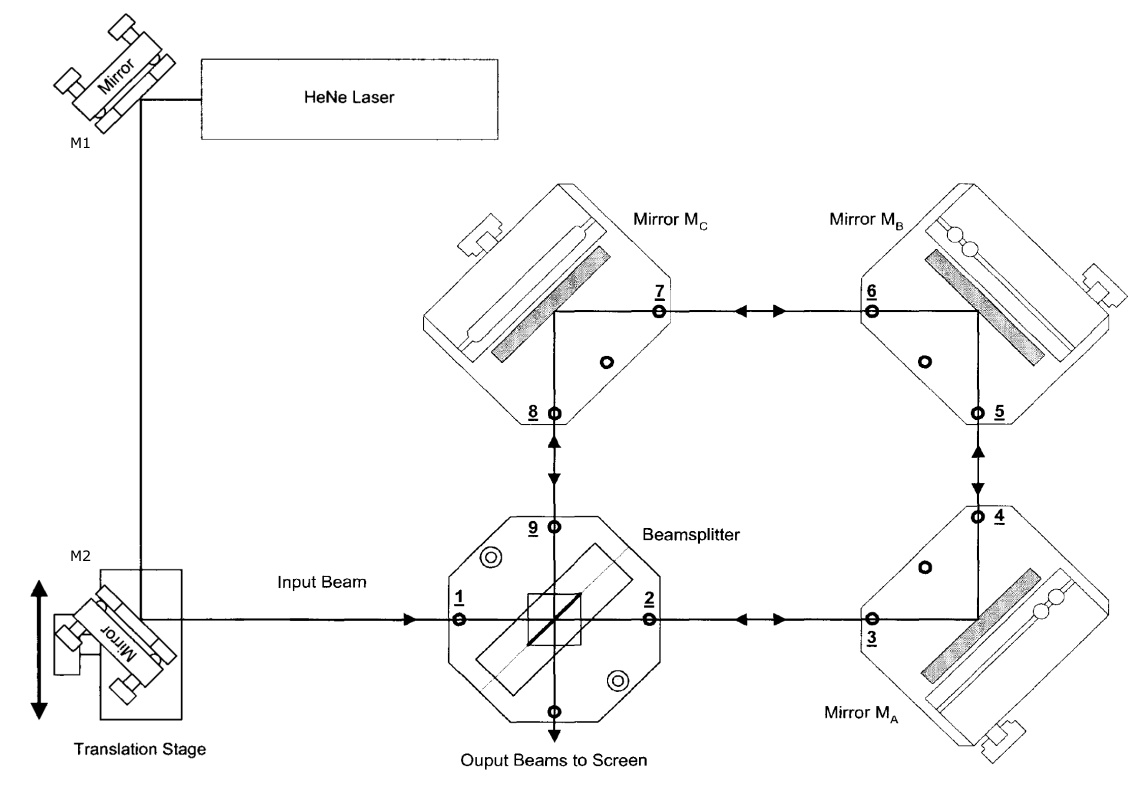
\includegraphics[width=0.9\textwidth]{img/aufbau_schematisch.png}
    \caption{Schematische Darstellung des Aufbaus eines Sagnac-Interferometers. \cite{sample}}
    \label{fig:aufbau}
\end{figure}
Eine schematische Darstellung des Sagnac-Interferometers ist in \autoref{fig:aufbau} dargestellt.
Als Lichtquelle dient ein HeNe-Laser, der linear polarisiertes Licht mit einer Wellenlänge von $\lambda = \qty{632.990}{\nano\metre}$ emittiert.
Über die Spiegel \textbf{M1} und \textbf{M2} wird der Lichtstrahl auf einen Strahlteilerwürfel (\textbf{PBSC}) gelenkt.
\\
Der PBSC erzeugt zwei orthogonal zueinander linear polarisierte Lichtstrahlen.
Ein Teilstrahl wird transmittiert und trifft auf Spiegel $\mathbf{M_A}$, ein weiterer Teilstrahl wird an der Grenzfläche des PBSC auf den Spiegel $\mathbf{M_C}$ reflektiert.
Bei optimaler Justage treffen die Teilstrahlen beide Spiegel mittig unter $\qty{45}{\degree}$ und erreichen anschließend den gleiche Punkt auf Spiegel $\mathbf{M_B}$.
Weiter werden die Teilstrahlen erneut auf den PBSC reflektiert.
Beide Strahlen verlassen den PBSC und können mittels Interfernzmuster auf eine Phasendifferenz untersucht werden.
\\
Sie durchlaufen also die gleichen Wege im Interferometer in entgegengesetzter Richtung.
Dies hat den Vorteil, dass beide Strahlen den gleichen Umwelteinflüssen, wie beispielhaft Luftdruckschwankungen ausgesetzt sind.
Das Interferenzmuster ist besonders stabil.

\FloatBarrier

\subsection{Aufbau zur Messung von Brechungsindizes}
Zur Messung von Brechungsindizes wird das in \autoref{sec:sagnac} beschriebene Sagnac-Interferometer verwendet.
In \autoref{fig:aufbau} ist eine Aufnahme des vollständigen Versuchaufbaus zu sehen.
Der Laserstrahl durchläuft einen Polarisationsfilter bevor dieser auf den PBSC trifft.
In einer Kontrastmessung wird der optimale Polarisationswinkel ermittelt.
Ziel ist eine gleichmäßige Aufteilung des vom Laser ausgesandten linear polarsierten Strahls in senkrecht und vertikale Anteile.
Dazu muss der Polarisationsfilter in einem Winkel von $\qty{45}{\degree}$ zu der Polarisationsebene des Lasers eingestellt sein.
Die Teilstrahlen weisen eine gleich hohe Intensität auf.
%ref SEC:kontrast  
\begin{figure}
    \centering
    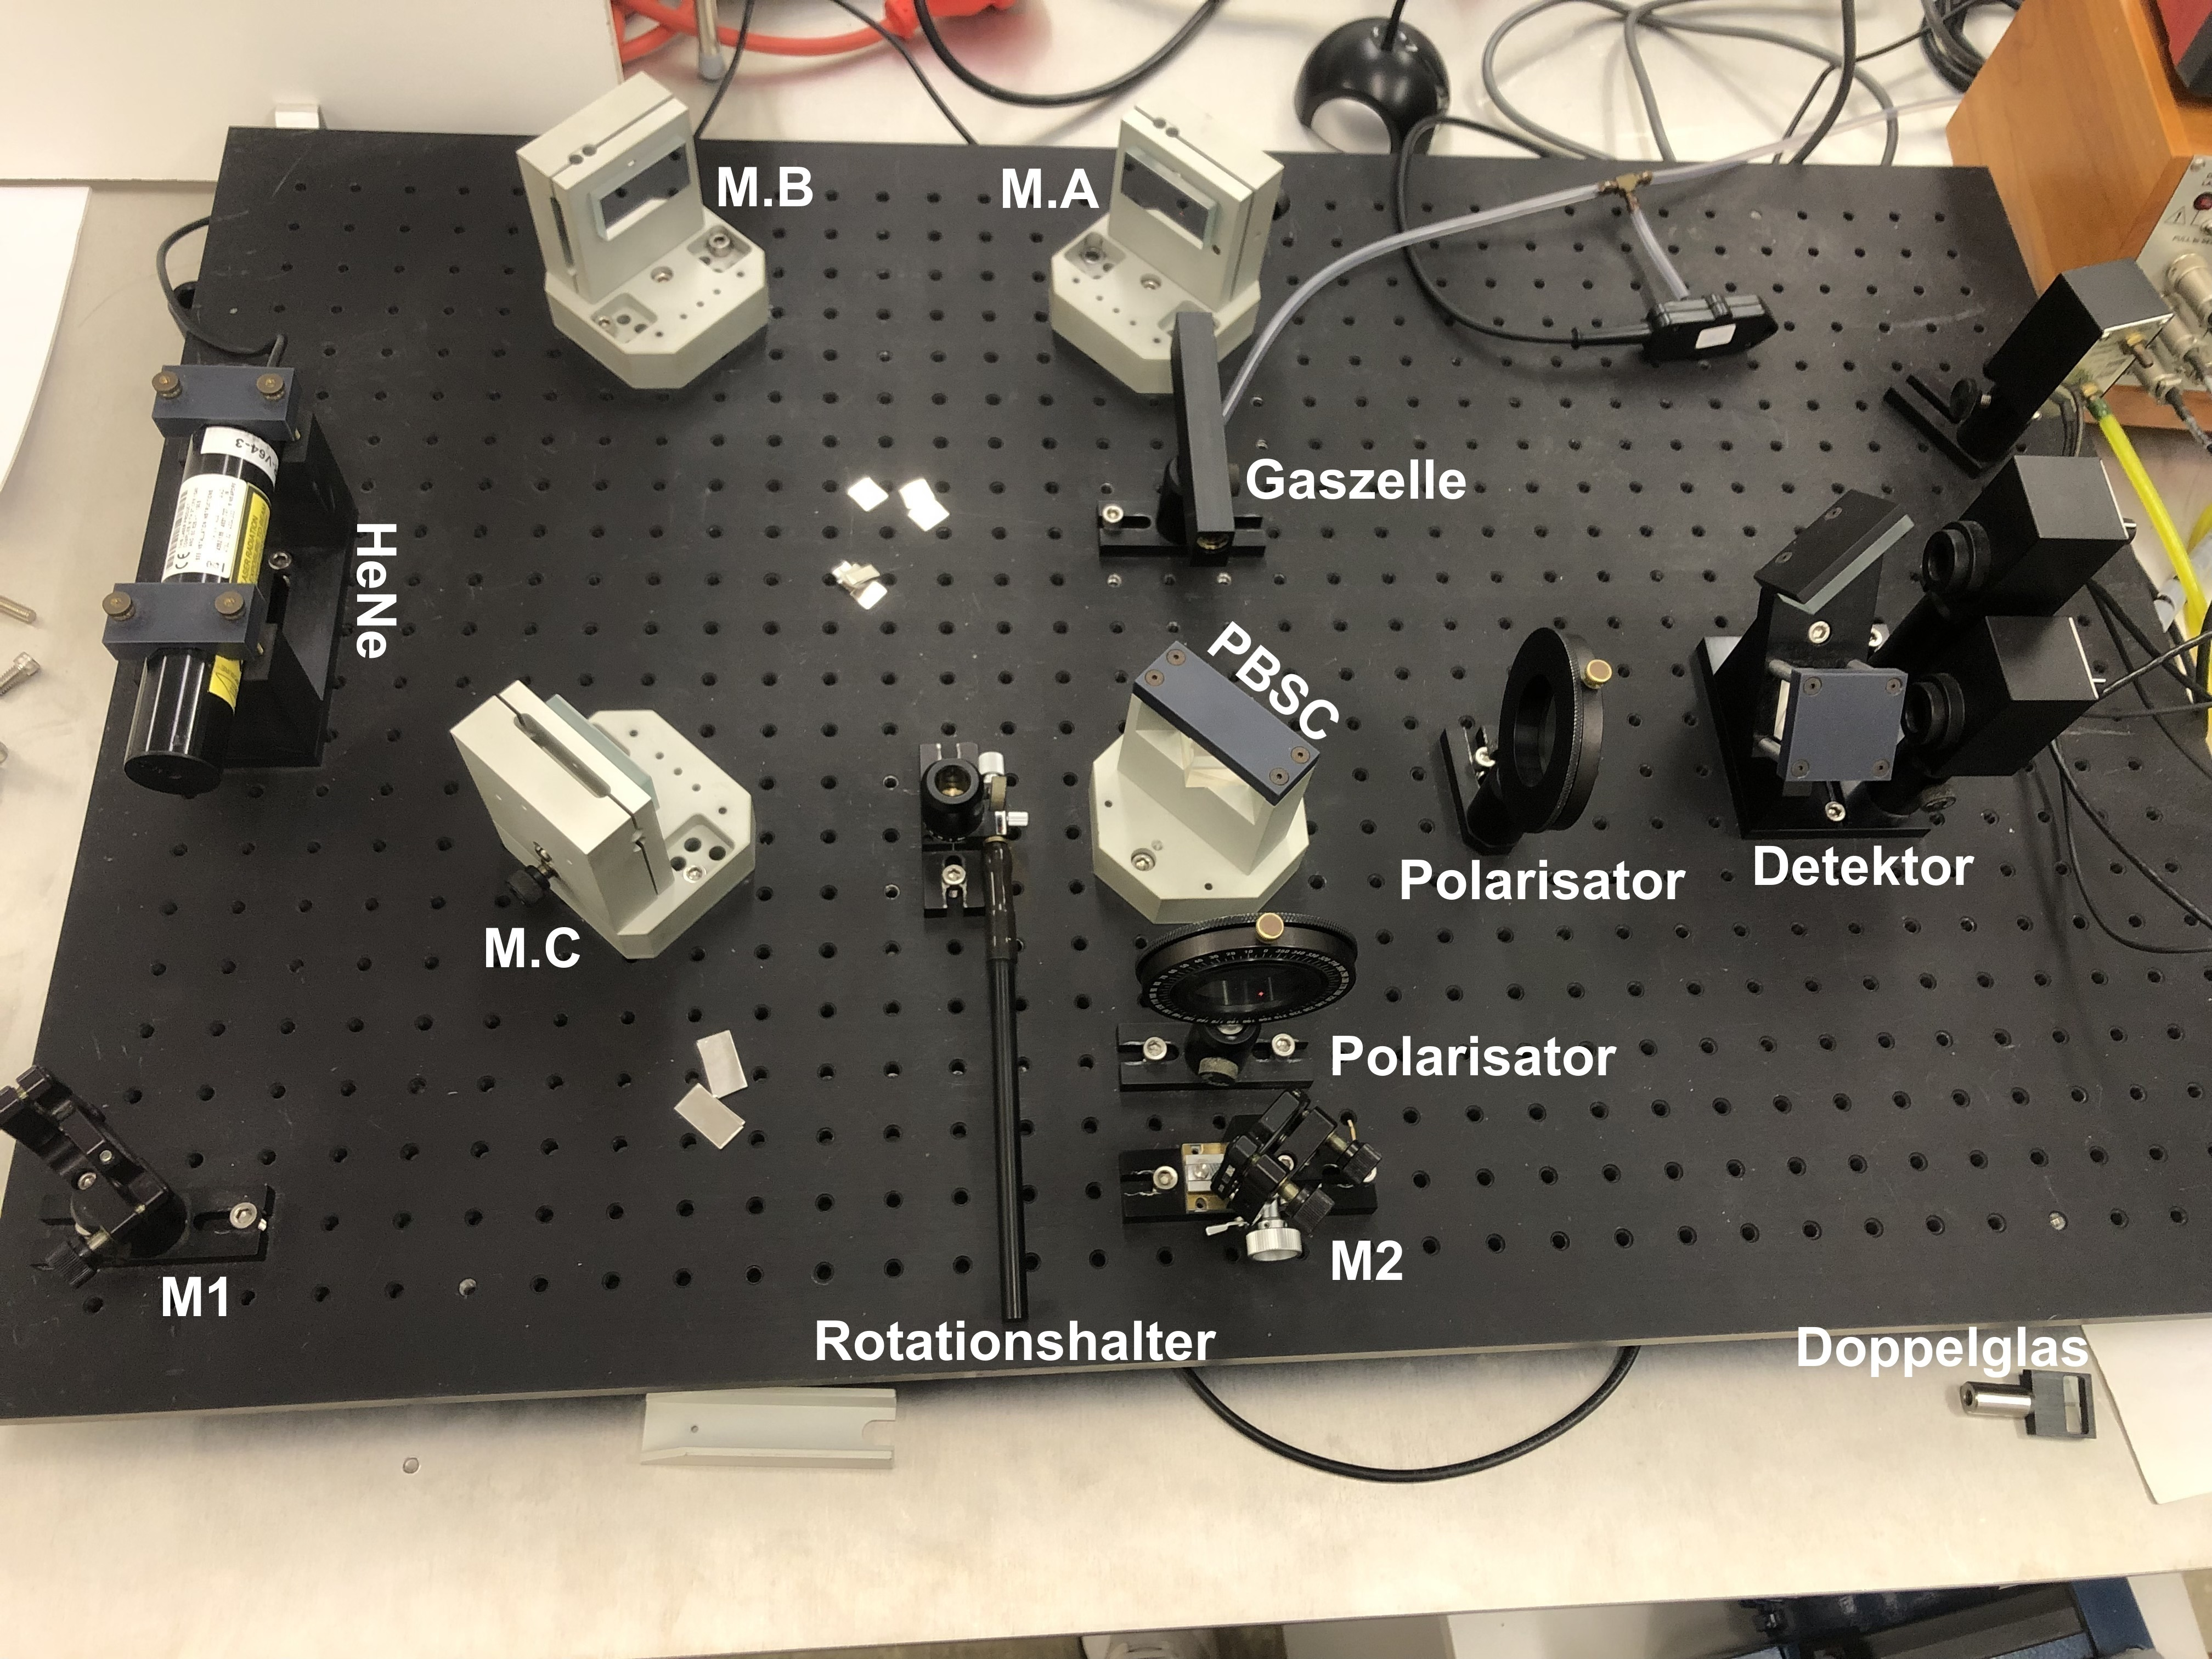
\includegraphics[width=0.8\textwidth]{img/aufbau2.jpg}
    \caption{Originalaufnahme des Versuchaufbaus mit einem Sagnac-Interferometer.}
    \label{fig:aufbau_original}
\end{figure}
Um im nächsten Schritt den Brechungsindizes einer beliebigen Probe zu bestimmten, müssen die beiden Teilstrahlen getrennt werden.
Dazu wird der Spiegel $\textbf{M2}$ parallel zu dem einfallenden Strahl verschoben.
Beide Strahlen durchlaufen nun getrennte Wege und treffen dennoch auf den gleichen Punkt im PBSC.
\\
Eine Gasprobe wird untersucht indem die Gaszelle in einen der Teilstrahle montiert wird.
Aufgrund einer kleineren Lichtgeschwindigkeit innerhalb des Gases benötigt das Licht eine längere Zeit um den gleichen Weg zurückzulegen.
Es kommt zu einer Phassendifferenz.
\\
Zum anderen kann der Brechungsindex von einem Doppelglas in einem Rotationshalter bestimmt werden.
Das Doppelglas besteht aus zwei Gläsplättchen die um $\pm \qty{10}{\degree}$ zueinander verkippt sind.
Dieses befindet sich im Rotationshalter, welcher um den Winkel $\theta$ gedreht werden kann.
Abhängig vom eingestellten Winkel durchlaufen die Teilstrahlen unterschiedlich lange Strecken im Glasplättchen.
\\
Das Fresnel-Arago-Gesetz (siehe \autoref{sec:polarisation}) sagt, dass zwei senkrecht zueinander linear polarsierte Strahlen nicht interferieren.
Für die Justage wird ein weiterer Polarisator unter $\qty{45}{\degree}$ in die Ausgangsstrahlen des PBSC platziert.
Auf einem dahinterstehenden Schirm sollte ein Interferenzmuster zusehen sein.
\\
Für die Messung der Brechungsindizes wird die Intensität des Lichtstrahls mit einer Photodiode bzw. bei der Differenzspannungsmethode mit zwei Photodioden detektiert.
Der Polarisationsfilter wird dafür durch einen zweiten PBSC ausgetauscht.
Beide Teilstrahlen des PBSC treffen jeweils auf eine Photodiode.
Die beiden Ausgangssignale der Photodioden können auf einem Osilloskop direkt sichtbar gemacht werden oder in ein Modern Interferometry Controller gegeben werden.
\\
Der Ausgang des Controllers ist proportional zu der Differenz der Eingangssignale und kann auf einem Oszilloskop abgebildet werden.
Konstante Störungen, wie externe Lichtquellen im Raum liefern bei der Differenzspannungsmethode keinen Beitrag.
Die Anzahl der Interferenzmaxima und -minima können so systematisch untersucht werden.